% chktex-file 44

\documentclass[a4paper,11pt]{article}
\usepackage[utf8]{inputenc}
\usepackage[russian]{babel}
\usepackage{geometry}
\usepackage{amsthm}
\usepackage[dvipsnames]{xcolor}
\usepackage{framed}
\usepackage{booktabs}
\usepackage{array}
\usepackage{amssymb}
\usepackage{adjustbox}
\usepackage{makecell}
\usepackage{float}
\usepackage{graphicx}

\definecolor{shadecolor}{RGB}{245,245,247} 
\geometry{left=2cm, right=2cm, top=2cm, bottom=2cm}

\title{Модель №.4. \\ Магнитные колебания. \\ Связанные маятники }
\author{Ким В.Р., Вишневский С.А \\ Группа M3207 }
\date{}

\theoremstyle{definition}
\newtheorem*{task}{Задание}\setlength{\parindent}{0pt}

\newenvironment{solution}
{\begin{shaded}\textbf{Решение:}\par\setlength{\parindent}{0pt}}
{\end{shaded}}

\newenvironment{answer}
{\par\noindent\textbf{Ответ:} }
{\par}

\begin{document}
\maketitle

\begin{task}
    Два одинаковых математических маятника, связанных пружиной с коэффициентом 
    жёсткости \(k\) на расстоянии \(L_1\) от точки крепления маятников. 
    Точки крепления обоих связанных маятников находятся на одном уровне. 
    Оба математических маятника имеют одинаковые длины подвеса \(L\) и массы \(m\) 
    (см. Рис.). 
    Сила сопротивления для каждого маятника прямо пропорциональна скорости. 
    Коэффициент затухания каждого маятника равен \(\beta\). Для заданных начальных 
    отклонений построить графики зависимостей углов и скоростей от времени 
    для каждого маятника. Найти нормальные частоты. 
    Параметры должны задаваться.

    \begin{figure}[H]
        \centering
        % 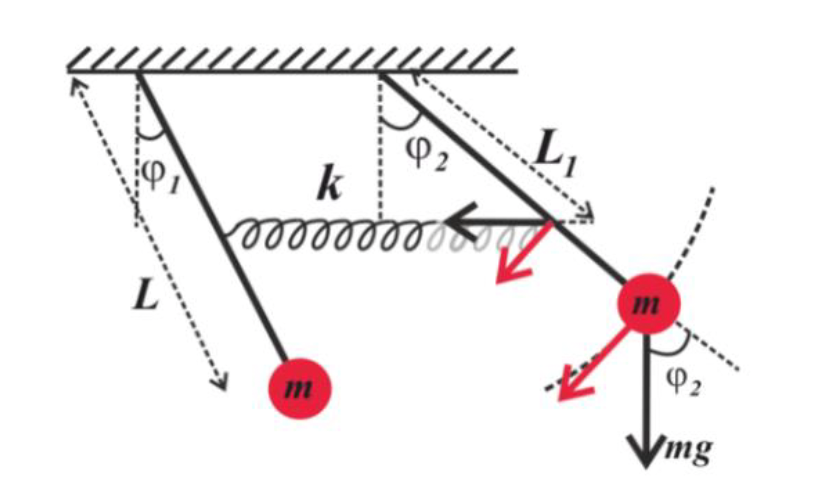
\includegraphics[width=0.5\textwidth]{"4. Connected pendulum/task.png"}  
    \end{figure}

\end{task}



Ниже представлено подробное описание теоретических основ, необходимых для моделирования системы 
двух связанных математических маятников. Все определения, формулы и рассуждения приведены с обоснованием 
их использования в численной модели.

\subsection*{1. Введение и постановка задачи}
Рассматривается система двух идентичных математических маятников, подвешенных на равной высоте, соединённых 
пружиной с коэффициентом жёсткости \( k \). Пружина прикреплена к маятникам на расстоянии \( L_1 \) от точки 
их крепления. Каждый маятник имеет длину \( L \) и массу \( m \). Для каждого маятника учитывается сила 
затухания, пропорциональная скорости, с коэффициентом \(\beta\). Целью задачи является построение графиков 
зависимости угловых отклонений и угловых скоростей от времени, а также определение нормальных частот системы.



\subsection*{2. Математический маятник: определения и базовые уравнения}
\textbf{Математический маятник} --- идеализированная модель, в которой масса сосредоточена в точке, а подвес 
считается нерастяжимым и безмассовым. Обобщённой координатой является угол отклонения \(\phi\) от вертикального 
направления (положения равновесия).

Для малых колебаний (при условии \(\sin \phi \approx \phi\)) уравнение движения выводится из закона 
сохранения момента импульса:
\[
\frac{d\vec{M}}{dt} = \vec{N},
\]
где \(\vec{M}\) --- момент импульса, а \(\vec{N}\) --- суммарный момент сил, действующих на систему.

Приводя это уравнение к скалярной форме для колебаний вокруг точки крепления, получаем:
\[
\ddot{\phi} + \omega_0^2 \phi = 0,
\]
где \(\omega_0 = \sqrt{\frac{g}{L}}\) --- собственная (естественная) частота свободного маятника, 
а \(g\) --- ускорение свободного падения.

При наличии затухающего сопротивления, пропорционального скорости, уравнение принимает вид:
\[
\ddot{\phi} + 2\beta\dot{\phi} + \omega_0^2 \phi = 0.
\]
Здесь \(\beta\) --- коэффициент затухания, отражающий диссипативные процессы в системе.



\subsection*{3. Система двух связанных маятников}
При рассмотрении двух маятников, связанных пружиной, следует учитывать взаимодействие, возникающее 
из-за разности их углов. Обозначим:
\[
\phi_1(t), \phi_2(t)
\]
--- углы отклонения первого и второго маятников соответственно.

В отсутствие затухания, уравнения движения можно записать следующим образом:
\[
\ddot{\phi}_1 + \omega_0^2 \phi_1 - \kappa^2 (\phi_2 - \phi_1) = 0,
\]
\[
\ddot{\phi}_2 + \omega_0^2 \phi_2 + \kappa^2 (\phi_2 - \phi_1) = 0.
\]
Здесь введён параметр связи \(\kappa\), который определяется через жёсткость пружины и геометрию 
системы. Часто встречается соотношение:
\[
\kappa^2 = \frac{k L_1^2}{mL^2}.
\]
Знак в членах, содержащих \(\kappa^2(\phi_2 - \phi_1)\), отражает то, что пружинная сила стремится 
уменьшить разницу углов маятников.

С учётом затухания уравнения дополняются членами, пропорциональными скорости:
\[
\ddot{\phi}_1 + 2\beta\dot{\phi}_1 + \omega_0^2 \phi_1 - \kappa^2 (\phi_2 - \phi_1) = 0,
\]
\[
\ddot{\phi}_2 + 2\beta\dot{\phi}_2 + \omega_0^2 \phi_2 + \kappa^2 (\phi_2 - \phi_1) = 0.
\]



\subsection*{4. Преобразование в нормальные координаты и нормальные моды}
Для упрощения анализа системы удобно ввести нормальные координаты:
\[
\xi_1 = \phi_1 + \phi_2, \quad \xi_2 = \phi_2 - \phi_1.
\]
Путём суммирования и вычитания исходных уравнений движения (без затухания для чистоты рассуждения) 
получаем:
\[
\ddot{\xi}_1 + \omega_0^2 \xi_1 = 0,
\]
\[
\ddot{\xi}_2 + \left(\omega_0^2 + 2\kappa^2\right) \xi_2 = 0.
\]
Таким образом, система сводится к двум независимым колебательным уравнениям с нормальными частотами:
\[
\Omega_{n1} = \omega_0 = \sqrt{\frac{g}{L}}, \quad \Omega_{n2} = \sqrt{\omega_0^2 + 2\kappa^2} = \sqrt{\frac{g}{L} + \frac{2kL_1^2}{mL^2}}.
\]

Решения для нормальных координат имеют вид:
\[
\xi_1(t) = \Phi_{01}\cos\left(\Omega_{n1}t+\varphi_{01}\right),
\]
\[
\xi_2(t) = \Phi_{02}\cos\left(\Omega_{n2}t+\varphi_{02}\right),
\]
где \(\Phi_{01}, \Phi_{02}\) --- амплитуды, а \(\varphi_{01}, \varphi_{02}\) --- начальные фазы, 
определяемые начальными условиями.

Переход обратно к углам маятников осуществляется по формулам:
\[
\phi_1 = \frac{\xi_1+\xi_2}{2}, \quad \phi_2 = \frac{\xi_1-\xi_2}{2}.
\]
В результате получаем общее решение для углов:
\[
\phi_1(t) = \frac{1}{2}\left[\Phi_{01}\cos\left(\Omega_{n1}t+\varphi_{01}\right)+\Phi_{02}\cos\left(\Omega_{n2}t+\varphi_{02}\right)\right],
\]
\[
\phi_2(t) = \frac{1}{2}\left[\Phi_{01}\cos\left(\Omega_{n1}t+\varphi_{01}\right)-\Phi_{02}\cos\left(\Omega_{n2}t+\varphi_{02}\right)\right].
\]



\subsection*{5. Режимы колебаний}
В зависимости от начальных условий в системе могут возникать различные режимы колебаний:

\begin{enumerate}
    \item \textbf{Синфазное колебание:} Если задать начальные условия так, что \(\Phi_{02}=0\), то
    \[
    \phi_1(t)=\phi_2(t)=\frac{\Phi_{01}}{2}\cos\left(\Omega_{n1}t+\varphi_{01}\right).
    \]
    Оба маятника движутся синхронно с частотой \(\Omega_{n1} = \omega_0\).

    \item \textbf{Противофазное колебание:} Если задать начальные условия так, что \(\Phi_{01}=0\), то
    \[
    \phi_1(t)=\frac{\Phi_{02}}{2}\cos\left(\Omega_{n2}t+\varphi_{02}\right),\quad
    \phi_2(t)=-\frac{\Phi_{02}}{2}\cos\left(\Omega_{n2}t+\varphi_{02}\right).
    \]
    Маятники движутся с частотой \(\Omega_{n2}\), но в противоположных фазах.

    \item \textbf{Суперпозиция нормальных мод (биения):} При возбуждении обеих нормальных мод, например, 
    если только один маятник изначально отклонён, решение для первого маятника может записываться как
    \[
    \phi_1(t)=\frac{\phi_1(0)}{2}\left[\cos\left(\Omega_{n1}t\right)+\cos\left(\Omega_{n2}t\right)\right].
    \]
    Применяя тригонометрическую формулу для суммы косинусов, получаем:
    \[
    \phi_1(t)=\phi_1(0)\cos\left(\frac{\Omega_{n1}+\Omega_{n2}}{2}t\right)
    \cos\left(\frac{\Omega_{n2}-\Omega_{n1}}{2}t\right).
    \]
    Здесь быстрые колебания с частотой \(\frac{\Omega_{n1}+\Omega_{n2}}{2}\) амплитудно модулированы медленной 
    огибающей с частотой \(\frac{\Omega_{n2}-\Omega_{n1}}{2}\) --- эффект биений. При слабой связи разность 
    частот невелика, а период биений оценивается как
    \[
    T_{\textnormal{биений}} \approx \frac{2\pi}{\Omega_{n2}-\Omega_{n1}}.
    \]
\end{enumerate}



\subsection*{6. Учет затухания в системе}
В реальных системах затухание приводит к экспоненциальному уменьшению амплитуд. Сила затухания для каждого 
маятника пропорциональна его скорости, поэтому к уравнениям движения добавляется член \(2\beta\dot{\phi}\). 
Итоговые уравнения с учетом затухания имеют вид:
\[
\ddot{\phi}_1 + 2\beta\dot{\phi}_1 + \omega_0^2 \phi_1 - \kappa^2 (\phi_2 - \phi_1) = 0,
\]
\[
\ddot{\phi}_2 + 2\beta\dot{\phi}_2 + \omega_0^2 \phi_2 + \kappa^2 (\phi_2 - \phi_1) = 0.
\]
Эти уравнения описывают, как затухание влияет на динамику системы, уменьшая амплитуду колебаний с течением времени.



\subsection*{7. Итоговая схема моделирования и интерпретация результатов}
При численной реализации модели на Python выполняются следующие этапы:
\begin{itemize}
    \item \textbf{Инициализация параметров:} вводятся значения \(m\), \(L\), \(L_1\), \(k\), \(\beta\), \(g\) 
    и начальные условия для \(\phi_1\) и \(\phi_2\).
    \item \textbf{Формулировка системы ОДУ:} записываются уравнения движения для \(\phi_1(t)\) и \(\phi_2(t)\) 
    с учетом затухания и пружинной связи.
    \item \textbf{Численное интегрирование:} для решения системы дифференциальных уравнений используются 
    численные методы (например, метод Рунге--Кутты).
    \item \textbf{Построение графиков:} полученные решения представляются в виде графиков зависимости углов 
    \(\phi_1(t)\), \(\phi_2(t)\) и их производных (угловых скоростей) от времени.
    \item \textbf{Определение нормальных частот:} на основании формул
    \[
    \Omega_{n1}=\sqrt{\frac{g}{L}}, \quad \Omega_{n2}=\sqrt{\frac{g}{L}+\frac{2kL_1^2}{mL^2}},
    \]
    вычисляются нормальные частоты системы, что позволяет дополнительно проанализировать режимы синфазных 
    и противофазных колебаний.
\end{itemize}

\subsection*{8. Заключение}
Представленная теоретическая база охватывает основные аспекты динамики двух связанных математических 
маятников с учётом затухания и пружинной связи. Были приведены определения математического маятника, 
обоснованы базовые уравнения движения, выполнено преобразование в нормальные координаты и получены 
выражения для нормальных частот. Описаны режимы синфазных и противофазных колебаний, а также эффект 
биений при возбуждении обеих нормальных мод. Эти положения лягут в основу численного моделирования 
системы на Python, что позволяет визуализировать динамику угловых отклонений и скоростей, а также 
исследовать влияние параметров системы на её поведение.

\end{document}
